% !TEX root = ./master.tex

\subsection{Le son et l'écoute}


Le son peut être déterminé par différents paramètres
physiologiques et psychologiques.
Il est défini très précisément par un ensemble d'unités physiques chiffrées
: les décibels  et les hertz. (Cf. Annexe)
Lorsque nous serons au chapitre concernant l'étude clinique,
ces quelques informations mises en annexe seront pertinentes pour la lecture des tests.

Lors d'un concert, si nous pouvions visualiser les sons qui
s'échappent de l'orchestre, ce serait un chatoiement de cercles qui se
répandraient tout autour de nous, comme
la propagation des
ronds dans l'eau suite à un ébranlement de sa surface.
Les molécules d'air en contact avec la source sonore se déplacent et
créent une vibration \autocite[183]{bencivelli:pourquoi,}.
Si la
musicothérapie a un impact certain sur la façon d'écouter en
entraînant sa
modification, peut-elle être  démontrée et démontrable, \textsl{objectivée},
simplement sous la forme d'un test, comme saisie par
l'\oe il neutre de l'objectif d'un appareil
photographique?

L'objet de notre étude débutera par la notion d'écoute que nous allons revisiter.
\subsection{Ecouter et entendre}
La définition du verbe `entendre' et du verbe `écouter'
nous paraît opportune
en raison de la confusion courante des deux termes.
\paragraph{Ecouter ou entendre : une différence}
\begin{quote}<<\,`Entendre', c'est  percevoir des sons, saisir par l'ouïe\,>>, tandis qu'avec
<<\,`écouter', on prête l'oreille à, on s'applique à entendre, on fait attention, on suit un avis, et \emph{au figuré}, on suit une impulsion, une inspiration\,>> \autocite[361--385]{hachette:dictionnaire} \end{quote}
Par les sources étymologiques du
terme `écouter',
 sa racine sanskrite \emph{ ``avih'' } se traduit par
 \emph{``évidence'' , ``connaissance'', ``discernement''}. Puis, en ancien
 français, ce mot a donné \textit{``ouïr''} signifiant aussi bien \textit{``entendre''} ,
\textbf{`` écouter'' } que \textit{``comprendre''} \autocite {etymologieWeb}:
 est-ce la raison
pour laquelle il subsiste toujours un amalgame en langue française
sur le sens de ce verbe?
De plus, par extension, \textbf{`` écouter'' }
permettrait non seulement de comprendre avec plus d'attention
mais aussi de percevoir des sons différemment, de manière plus particulière, douée d'une forme de
\textit{``clairaudience"}, (faculté d'audition paranormale) selon Didier
Colin \autocite {colin2015}.

En définitive, \emph{`entendre'} est une attitude passive par rapport au monde sonore
qui nous entoure. Nous recevons les sons sans les interpréter, sans
effort, étant une action involontaire, non
sélective. Plus simplement, on
\begin{quote}
	<<\,suppose un son (physique), une oreille
	pour le capter, un système nerveux pour le recevoir.\,>>\autocite[2]{auriol:cle}
 \end{quote}
 Tandis qu'\textit{`écouter'}
\begin{quote}
	<<\,est un
	processus actif supposant préférences et répulsions pour tel son ou
	telle séquence sonore.\,>>\autocite[2]{auriol:cle}

\end{quote}
Entendre et écouter sont donc  «\,deux
fonctions essentiellement distinctes bien qu'évoluant apparemment sur
des terrains iden\-ti\-ques\,>>
% ancien texte {\textbf{site internet: http: auriol.free.fr} Extrait de l'entretien réalisé par
%	Bernard Auriol avec Alfred Tomatis, 1973.}.
[\dots] avec «\,l'é\-lé\-ment cons\-cient, facteur essentiel sur lequel repose toute la
différence entre ces deux activités\,». \autocite[122]{tomatis_oreille_1991}
Remarquons bien qu'
\begin{quote}

	<<[\ldots] \emph{Entendre, c'est en quelque sorte subir
		un son} ou un message qui nous est adressé. \emph{Ecouter, c'est désirer appréhender ce son} ou ce message [\ldots]>>
	\autocite [p. 111]{tomatis:education}.
\end{quote}
Selon B. Auriol \autocite[18] {auriol:cle} et Tomatis \autocite[52]
{tomatis:loreille}, l'\textbf{écoute} est un `` éveil auditif''  défini avec au
minimum trois
fréquences simultanées (dans le sens esthétique). Il s'agit donc d'un phénomène
complexe avec la corrélation d'axes
linéaires (notion temporelle) et verticales (notion spatiale), doublée d'une
dimension psychologique.
En effet, si \enquote{\emph{Je suis la musique que je fais ou écoute}}
\autocite [8]{viret:b}, \textbf{écouter} implique une conscience pour s'actualiser dans le sujet.
Elle est une opération
qui suppose une participation active dans le choix du message
ou dans la sélection d'une voix. Elle  implique la volonté,
\pdfmargincomment[color=green]{Bien!}
permet une forme de décodage:
si nous nous trouvons dans une ambiance sonore à fort volume, pour
parvenir à lire, nous
ferons abstraction des bruits environnants tout en en ayant
conscience, parvenant à nous en extraire pour focaliser notre
attention sur cette lecture. Nous parvenons à couper les sons parasites, à nous en abstraire pour
nous concentrer uniquement sur les plus  pertinents. Et ceci se fait grâce à cette capacité si importante
d'\textbf{écoute} en connection avec notre cerveau.
%Dans un milieu sonore important,
% bruyant, comme un café, lorsque nous lisons attentivement, nous faisons abstraction
%des bruits environnants; en soi, nous les entendons parfaitement mais nous n'y
%prêtons pas attention.
Puisant encore davantage dans  la racine de ce mot, ``écouter'' signifirait
aussi \emph{partager}, ce qui prend tout son sens lors d'un dialogue ou
pour la voix (supposée, imaginée) de  l'écrivain qui
 chante à travers un livre avec celle, intérieure, du lecteur.
 % phénomène se réalise avec un livre qui transmet et partage des
  %connaissances. L'écoute permet donc la communication, sous-entend le
 % plus souvent la présence d'un être en vis-à-vis et nécessite de la
 % concentration. Il faut cette volonté inclue dans celle-ci  pour
 % comprendre et rentrer en contact avec la voix de  l'écrivain qui
 % chante dans le texte avec celle, intérieure, du lecteur.


  \textbf{Ecouter} se base ainsi certes sur une stimulation prenant sa source à
l'extérieur mais devant être \textbf{ intérieurement et intentionnellement
	recherchée}:

  Vouloir voir, c'est viser, vouloir entendre, c'est
      écouter.
  L'\oe il regarde par la rétine et  vise, sous l'ordre du
  cerveau, avec la macula. Dans la même idée, par l'écoute,
  l'oreille et la cochlée (partie interne de l'oreille) permettent
  l'analyse des sons. Vouloir entendre dans le but d'écouter est comparable  à
  la visée de l'\oe il lorsque l'on veut collecter une
  information.
   Ainsi, l'audition est la capacité perceptive du système auditif et l'écoute, c'est ce qu'on en fait.


      \textbf{Ecoute musicothérapeutique}:


Qu'est-ce qu'une écoute dite musicothérapeutique? le sujet est vaste, mais nous voulons faire un rapide lien avec le concept de 'communication' abordé plus haut.



Car nous pouvons aussi différencier des différents types d'écoute. D'après Edith Lecourt \autocite [182] {lecourt:decouvrir},
%\footnote{ <<\,De l'écoute verbale à l'écoute musicale\,>>},
%\[ch. 10 <<\,De l'écoute verbale à l'écoute musicale\,>>, p. 182.]
on en distingue plusieurs : l'écoute verbale, musicale, plurivocale et multiple.
 L'analyse musicale qui permet la différenciation d'une voix d'un ensemble polyphonique est appelée \emph{plurivocale}. Celle qui est multiple n'est pas analytique  mais
 \begin{quote}
 	 [\ldots] \textit{ouvre une disponibilité, met en suspens les grilles verbale et musicale} [\ldots] \emph{pour parcourir le vécu sonoro-affectif}\autocite[183]{lecourt:decouvrir}.
 \end{quote}
 Employée en musicothérapie, elle la nomme la technique de la  \emph{communication sonore} qui peut apporter
 <<\,des ouvertures sur l'analyse des niveaux plus archaïques de l'organisation mentale\,>>\autocite[154]{lecourt:decouvrir}.
 Par l'expérience musicale en groupe, Anzieu cite un moment
 particulier, de ``grâce"  nommé ``le concept d'illusion groupale" \autocite[113]{AnzieuMoiPeau},
 l'illusion d'une unité absolue, comme un seul corps .








\paragraph{Ecoute objective ou subjective?}

\emph{L'écoute} implique donc les notions de \emph{son} et
d'\emph{oreille}. Leurs définitions et caractéristiques physiques, bien qu'importantes, ont été mis en
annexes ainsi que les détails
d'anatomie. (Cf. Annexe 1.: Son et Oreille.)
La compréhension de ces aspects nous
permettra de mieux situer notre travail et les hypothèses y afférentes.


Nous avons tous,
selon les manuels d'anatomie, la même
oreille, du moins nous pouvons reconnaître une analogie de structure. Nous devrions donc entendre et écouter la même chose
lors d'une même information diffusée tout comme le fait un enregistreur avec un micro. Pourtant il n'y a pas d'écoute \emph{passive}. Chacun n'entend pas de la même manière les mêmes
informations, chacun trie et fait son propre choix selon la fonction
d'écoute élaborée depuis l'enfance. Cette fonction sélectionne très
rapidement les mots pour être intelligible, pour se faire
comprendre. Nous rejoignons l'idée de Tomatis lorsqu'il affirme que
\textit{"L'oreille a un psychisme"}, car tout un chacun entend ce qu'il veut bien
entendre \autocite [167]{tomatis_oreille_1998}.
Nous transformons notre écoute selon nos attentes.
Allant dans le même sens, cet
article d'une
étude franco-américaine \autocite{lemonde.fr:stradivarius} au sujet des célèbres violons
Stradivarius: faite avec un protocole
d'écoutes en aveugle avec
des violonistes professionnels et en parallèle avec un public (caché
derrière un rideau), elle démontre que le mythe de la suprématie
de ces instruments extrêmement chers tombe au profit d'instruments
neufs.

Le cerveau
transforme les informations reçues selon nos attentes et joue un
rôle majeur dans notre perception.
\autocite%[43]
{roque:lecoute}.
%
%\footnote{\href{http://www.lemonde.fr/culture/article/2014/04/10/le-stradivarius-detrone-par-les-violons-modernes\_4398681\_3246.html}{LeMonde.fr}.}.
\subsection{La perception des sons et l'existence de troubles
  émotionnels}
De manière générale, ce pouvoir du cerveau a transformer nos capacités d'écoute en sélectionnant les informations nous interpelle, notamment au sujet des  patients ayant participé à cette étude.
Que se passe-t-il en pleine
souffrance émotionnelle? Ces souffrances sont-elles dues à des situations
insupportables qui
ordonnent justement à notre cerveau de se protéger en obscurcissant la
perception sonore?  Ne plus vouloir écouter certains
sons permettrait-il en quelque sorte d'échapper à la souffrance et de faire une
pause dans la douleur? Nous avons le droit -- et c'est un réflexe de
survie -- de ne pas vouloir assister à une scène insupportable et de détourner
notre regard.  Nous pourrions supposer qu'il en est de même pour l'oreille ne voulant plus capter
certains sons. C'est une fermeture aux sons, une création d'une coque ou d'une bulle protectrice. En d'autres termes, il s'agit d'une \textbf{distorsion} dont nous reparlerons au chapitre 3.
Freud mettait déjà en évidence le phénomène de la
\textbf{sélectivité } comme ``mécanisme de défense'' \autocite{ Freud}.













\paragraph{ L'écoute dans le rapport
  musique-cerveau}
Ce qui précède atteste de la très grande complexité de notre cerveau.
Voyons brièvement ce qu'il en est des incessantes recherches scientifiques actuelles.
  %Conformément à l'idée que l'oreille nécessite d'être sollicitée pour
  %énergiser le corps et le cerveau en vue d'un épanouissement, la
  %capture d'un très grand nombre de stimulations par seconde agit
  %sur la \gls{réticulée} (Cf. Glossaire ),
  %%%(Cf. Glossaire)

Signalée depuis la plus haute Antiquité,  la reconnaissance de
l'impact de la musique sur l'émotion est actuellement confirmée par
des approches récentes: Damasio
%\footnote {{L'erreur de Descartes}, Antonio Damasio, Paris,  Ed.Odile Jacob, 1997},
souligne l'indispensable effet de l'\textbf{émotion}
sur l'intelligence   ---     \textbf{intelligence émotionnelle et intelligence
  cognitive} --- \autocite {damasio:lautre}.
En outre, les approches neuro-psychologiques sur les \textit{agnosies
  auditives} \autocite[205--216]{seron.baron.ea:neuropsychologie},
sur la perception distincte des émotions de la musique
\autocite[223--224]{platel_neuropsychology_2002},
sur l'apport de Bigand  \autocite {bigand:cerveau}
%\footnote {Bigand E., chercheur, professeur
%de psychologie cognitive à l'Université 2013 }
soutenant le
manque de fonction biologique précise de la musique,
et sur la
découverte du rôle mimétique des\textit{ neurones miroir }( ``troisième''
cerveau) par Rizzolati \autocite{Rizzolati} en 1990.
% relatée par Van Eersel.
%\autocite[118--119]{van_eersel_cerveau},
%\footnote{"Notre cerveau n'a pas fini de nous étonner", Entretien
%avec Jean-MichelOughourlian, Ed. Albin Michel, Le Livre de Poche 2012}
Toutes ces recherches soulignent cette relation constante entre cerveau et musique.


Quant au \textbf{ lien entre audition et troubles de l'humeur}, comme souffrent
les patients testés, d'autres perspectives
récentes mettent en lumière les évaluations de ces dernières recherches  comme les approches de Yowell \autocite{Yowell},% Sackheim & Epstein et al.
%\footnote{Yovell
%  Y., Sackeim, H.A., Epstein, D.G., Prudlic, J., Devanand, D.P.,
%  McElhiney, M.C., Settembrino, J.M. Bruder, G.E., 1995. Hearing loss
%  asymmetry in major depression. J. Neuropsychitr. Clin. Neurosci. 7,
%  82--89.}
%  Millot and Brand (2001) et
Canbeyli \autocite{Canbeyli},
%\footnote{Canbeyli R., 2010. Sensorimotor modulation of mood and
%depression: a integrative review.Behav.Brain.Res. 207 (2), 249--264}
études citées dans celle d' \autocite{affectiveDisorders}. Toutes soulignent
l'important\textbf{ lien entre la difficulté}
à \textbf{percevoir certains sons et la présence de troubles émotionnels,}
laissant entendre une correspondance sous forme de `` vase communiquant''
entre la \textbf{perte de reconnaissance de
sons et un état dépressif.}

Cette étude, \autocite{affectiveDisorders}, faite
%\footnote{``Les seuils auditifs des sons purs
%	sont diminués chez les personnes déprimées avec des
%	troubles de stress post-traumatique.'', <<\,Pure-tone auditory
%	thresholds are decreased in depressed people with post-traumatic stress
%disorder\,>>	.}
   en collaboration avec
le CNRS de Marseille (Centre National de Recherche Scientifique)
 mentionne \textbf{l'effet des événements
traumatisants sur l'audition}, impliquant des conséquences dépressives:
la double approche groupale (Gr en bonne santé et Gr déprimé avec
troubles de stress post-traumatique) met en lumière \textbf{la diminution des
  seuils auditifs}. (Cf. Test clinique, ch.6 p. 44)
C'est ainsi que l'on relève une augmentation de l'activité de la
première aire projective primaire et deuxième aire auditive (aire
secondaire associative) ainsi qu'une diminution significative des
seuils auditifs par voie osseuse, et plus précisément entre
\SIrange{275}{8000}{\Hz}) et en conduction aérienne
(\SIrange{500}{875}{\Hz} et  \SIrange{2000}{8000}{\Hz}.

Sans nous éloigner trop de notre sujet, nous pouvons rappeler
les difficultés observées sur les
\textbf{autistes} et leur capacité d'écoute cérébrale excessive et
incontrôlable investiguées par Harrisson et St-Charles \autocite {harrisson_autisme_2017}\footnote{Cet ouvrage propose une description unique du TSA
   (trouble du spectre de l'autisme
   pp. 22--23)}. Dans ce tableau
 figure un trouble d'intégration sensorielle (TSA), où
 \textbf{l'hypersensibilité aux sons} devient douloureuse quand le flux excessif
 des
 informations empêche le tri, protégeant ainsi le cerveau d'une surcharge.

\paragraph{Rapport entre audition et émission vocale}

%Le rapport entre audition et émission vocale
%est enrichi par les travaux de
 %\footnote{psychologue, formateur
%Tomatis, (Paris), co-auteur de l'étude CNRS des seuls auditifs et
%dépressifs

Granier, co-auteur de l'étude \autocite{affectiveDisorders} précédemment citée, poursuit les travaux de Tomatis et soutient également qu'\textit{ ``il existe une
interaction
constante entre  \textbf{le traitement auditif et moteur de la
voix}, soit entre l'information sensorielle et les programmes moteurs impliqués
dans la parole ou le chant.''}.
% propos issus de la formation continue, avril 2012, Paris, Granier.
Le programme moteur qui a été déclenché
pour la parole permet au cerveau d'effectuer des tentatives d'anticipation
des émissions acoustiques imminentes, comparées à l'information
auditive reçue; cette boucle
auditivo-vocale/ verbale permettra, dans un processus circulaire, un ajustement,
et par là même, comme l'enseignait Tomatis, une mise en \textbf{résonance}.

Ainsi, le concept de \textbf{`résonance'} s'applique non seulement aux instruments mais aussi au corps humain. Les ondes sonores pénètrent dans nos cellules et entrent en résonance vibratoire. L'être humain ressemble à un instrument de musique complexe, unique et accordé.
Les travaux de Sigrist au sujet du burnout ont permis de faire un lien étroit avec la problématique de la
 \textbf{résonance}, dite \enquote{\textit{Resonanzstörung}}.
%Le nombre limité d'études musicothérapeutiques au sujet du \textbf{burnout}
%nous invite aux travaux de Sigrist F., \autocite[pp.55--90] {sigrist_burnout_2016}
%parlant de \textit{``Resonanzstörung''}
L'auteur y relève la connection neuronale
directe et significative entre les systèmes auditif et
         limbique, d'où découle une activation émotionnelle et une
         \textbf{résonance} définie comme
         ``interpersonnelle'',\enquote{\textit{interpersonnelle
             Resonanz} }\autocite[55--90] {sigrist_burnout_2016}.
             % F. Sigrist, médecin
%psychiatre, psychologue et musicothérapeute à la Privatklinik
%d'Hohewegg, Zürich.
Propos appuyés en l'occurence par \textbf{la neuroscience sociale} \autocite[201]{van_eersel_cerveau}:  cette nouvelle discipline émerge depuis
les années 1990 (Cacioppo J. et Berntson B.) et greffe à "l'intelligence
émotionnelle" celle dite "relationnelle", affirmant et confirmant ainsi la nécessité vitale pour
 \textbf{nos neurones  de rentrer en \textit{résonance} avec d'autres neurones.}


 Cette relation constante entre cerveau et écoute,
ce lien puissant et indissociable, est attestée par toutes ces recherches et nous permet d'aller dans
 le sens de notre étude tout en appuyant
 la fonction thérapeutique de la musique.


En effet, l'écoute peut être fragilisée, modifiée, distordue, appliquant une sélection de sons par la mise en place du cerveau d'un \enquote{système d'évitement} \autocite {Kabat-Zinn}.
Lorsqu'une mise en résonance est activée, la prise de conscience peut avoir lieu, ce qui permettra une forme de restauration des données.
Nous y reviendrons au chapitre de la discusion et des conclusions.










\chapter{Tests musicothérapiques}
%Avant d'aborder le test d'écoute qui va nous intéresser plus
%particulièrement pour notre travail, nous allons faire la différence
%entre la définition du test et celle de l'épreuve.
%Le test est normé, c'est une épreuve codifiée, numérisée, échelonnée,
%statistifiée, comme celui du test d'intelligence de Piaget où il y a une
%norme et des chiffres. Tandis que l'épreuve est plus globale, plus complexe,
%demande plus de matériel et permet de
%cataloguer mais n'est pas statistifiée.

%Selon le dictionnaire de psychologie \autocite {doronparot}, c'est en 1890 que le test (du latin ``testum''
%signifiant ``pot de terre'') a été utilisé pour la
%première fois. C'est un procédé d'évaluation qualitative ou
%typologique des caractéristiques d'une substance, d'un corps et d'une
%fonction.
%Le test psychologique est une épreuve définie impliquant une tâche à
%remplir, identique pour tous les sujets examinés, avec une technique
%précise pour l'appréciation du succès ou de l'échec.
%L'épreuve (action d'éprouver) est ce qui permet de juger la valeur
%d'une idée, d'une qualité intellectuelle ou morale d'une personne.

%La psychologie clinique s’intéresse moins
%aux tests et plus aux à-côtés des tests, c. à d. aux réactions de la
%personnalité à la situation à la fois matérielle et sociale dans
%laquelle le sujet se trouve placé. L’épreuve spéciale analytique,
%quantitative, ne prend tout son sens que rapprochée d’autres épreuves
%analogues (comme dans le profil psychologique) intégrée dans le
%portrait psychologique global.

%Cette réciprocité de l’ensemble et du détail est une condition générale de la psychologie humaine : sur l’intuition d’ensemble initiale quelques faits particuliers viennent se profiler, l’image de l’ensemble est révisé et permet d’interpréter de nouveaux détails ; d’autres détails modifient à nouveau l’ensemble, et ainsi de suite.


%L’analogie est frappante avec la médecine clinique : là aussi on a
%espéré substituer à l’art clinique incertain une somme d’examens de
%laboratoire ; mais là aussi il a fallu revenir à l’idée d’une
%intégration des examens de laboratoire dans l’ensemble clinique.
Nous nous sommes intéressés à rechercher le sens du mot "test'' puisqu'un appareil spécifique nous a permis de le faire pour ce travail. Quelle est sa définition, son utilisation globale et quelles sont les différences observables?
Est-ce un test audio, musico, psychologique?
Quels sont les types de tests utilisés en musicothérapie?
%Qu'appelle-t-on test dans ce dans ce domaine?
Raisons pour lesquelles nous avons recherché son origine, évalué les différences entre la psychologie et le médical, listé un éventail des tests dénommés bilans musicaux en musicothérapie, alliant psychologie et musique.


\section{Test d'écoute et audiogramme:}


A l'origine et selon le dictionnaire de psychologie \autocite {doronparot}, c'est en 1890 que le mot "test" (du latin ``testum''
signifiant ``pot de terre'') a été utilisé pour la
première fois. C'est un procédé d'évaluation qualitative ou
typologique des caractéristiques d'une substance, d'un corps et d'une
fonction.

Généralement, la dénomination de \textbf{test d'écoute} se trouve sous forme verbale,
à caractère
\textbf{psychologique}, mettant principalement l'accent sur la communication
et la capacité d'empathie.


Par contre, dans le milieu médical, on le nomme non pas test d'écoute mais test d'audition ou \textbf{audiogramme}, test servant à mesurer les seuils d'audition des sujets, grâce à l'audiomètre. Cet
appareil français avait été mis au point en 1933. Les Américains
ont repris ces travaux pendant la dernière guerre pour pouvoir dépister
les dommages subis par ceux qui conduisaient des avions ou d'autres
engins similaires bruyants.
Ainsi l'audiogramme est une épreuve d'ordre \textbf{physiologique} et peut faire partie des examens  pratiqués en otologie
%\footnote{otologie : branche de la médecine qui étudie l'oreille et ses maladies.}
pour poser un diagnostic.
   C'est un examen à partir duquel se
  dessinent les données dénommées étiologiques
  %\footnote{étiologie : étude des causesd'une maladie}
  pour détecter un trouble de la fonction auditive. Un pronostic pourra définir le mode de thérapie
médicale, chirurgicale, prothétique ou rééducative avec une procédure
technique incluant des paramètres et manipulations propres au corps
médical des auscultations O. R. L.


\section{Les tests d'écoute en musicothérapie}
\label{musicothEtpsycho}
Les musicothérapeutes ne se lassent pas d'explorer l'alliage du son
 et de la psychologie, et inversément, les psychanalystes, les psychiatres, les psychologues
 s'intéressent à intégrer le son dans leur travail. Par ce truchement,
 une élaboration est faite, porteuse d'informations différentes que
 celles d'un questionnaire médical. Le son permet de donner un miroir
 psychologique de la personne par un chemin détourné.

La musique s'est révélée ainsi être un important support
         d'expérimentation.   \textbf{Benenzon} \autocite{benenzon:musicotherapie},\textbf{ Verdeau-Paillès} \autocite{verdeau-pailles:bilan} et
         \textbf{Lecourt }\autocite{lecourt_les_2017}
         % \textbf{Bonny} \autocite{bonny_gim}
         ont su intégrer dans leur pratique l'utilisation du\textbf{ son }comme
         élément facilitant l'exploration psychique et
         ont, chacun à leur manière, élaboré des procédures destinées à faciliter
         l'introspection et la communication.


         A proprement parler, avec le terme "test" en musicothérapie, il en existe deux types, le réceptif et l'actif. Il ne s'agit en aucun cas de tester des compétences musicales mais de \enquote {définir un type de sensibilité et des traits de personnalité}.\autocite[83]{lecourt_les_2017}.
Le test réceptif, mis à part les recherches que cite Lecourt à partir de \enquote {réactions aux bruits et sonorités (G. Boissière), aux rythmes (C. Holthaus) ou aux intervalles musicaux (le Savioz PPIT sur une base jungienne)} \autocite[83]{lecourt_les_2017}, le test réceptif reste dans sa globalité réalisé à partir d'oeuvres musicales, protocole qui avait été mis au point avec Jacques Jost, technicien du son et pionnier en la matière dès 1954 \autocite{Jost}.
         Le test actif, de son côté, évalue la créativité, les possibilités d'expression du sujet par l'intermédiaire d'un instrumentarium. Ces deux types  de tests vont peu à peu se réunir pour former
                 le \textbf{ bilan
                     psycho-musical}.
%(2017)\autocite[p.~84]{lecourt_les_2017}


C'est à \textbf{Jacqueline Verdeau-Paillès} neuropsychiatre,
  musicothérapeute à Limoux (France) (1924-2010) que l'on doit le premier bilan
                     psycho-musical en 1980 qu'elle a réalisé avec ses patients dans son service
                     de psychiatrie à Limoux.
L'ouvrage \enquote {\textit{Le bilan musical et la personnalité}}\autocite{verdeau-pailles:bilan}
                     est un outil qui permet, en partant des \enquote {liens personnels avec le sonore}, d'obtenir des \enquote {critères objectivables} précise l'auteur  \autocite[37]{vrait_musicotherapie_2018}, pour évaluer la disponibilité du sujet pour cette
                     approche et permet au thérapeute de l'orienter dans
                                 une telle prise en charge. En premier lieu, un entretien constitue \enquote {\textit{la fiche de réceptivité musicale} } avec un \textbf{test} de 10 extraits musicaux, choix standardisé après évaluation réalisée auprès de nombreux auditeurs--, oeuvre descriptive, insolite, affective etc.
Puis, avec l'analyse des verbalisations, un \enquote { \textit{psychogramme de réceptivité musicale} } est établi en classant les réponses sensorielles, cénestésiques, motrices, etc. Enfin, suit \enquote {\textit{le \textbf{test}  psychomusical actif} } \autocite{verdeau_expression} de courte durée (10') avec une observation minutieuse des réactions comportementales, des capacités créatrices et relationnelles et l'analyse des productions sonores. Puis, en  dernier lieu, intervient la synthèse du bilan psychomusical, ce qui permettra d'amplifier la palette d'éléments
                                cliniques et anamnestiques, facilitant ainsi un meilleur approfondissement du
                                 contenu extériosé en activant aussi l'aspect artistique.
Notons que le dépouillement des tests réceptifs est réalisé, nous fait remarquer Lecourt, avec un musicothérapeute et l'aide d'un professionnel habilité aux \enquote {techniques projectives, protocole inspiré du Rorschach et du TAT, afin d'obtenir un tableau de résultats tirés de catégories de "réponses "simples", "complexes" et "défensives"}\autocite[p.86] {lecourt_les_2017}.

C'est avec Verdeau-Paillès que la conception de la musicothératie va radicalement évoluer pour se centrer sur le patient et l'introspection que le \textbf{test} suggère.

 Durant cette même période, années 70-80,
\textbf{ Rolando Omar Benenzon} psychiatre, psychanalyste,
musicien et musicothérapeute, né en 1939 à Buenos Aires a également élaboré une technique similaire au \enquote {\textit{test psychomusical actif} }de Verdeau-Paillès,
 où une co-influence n'est pas à exclure.
 En effet, avec Benenzon, sa définition de la musicothérapie comporte
\emph{\textsl{ ``les expressions corporo-sonoro-non
     verbales''}}, \autocite{benenzon:musicotherapie},
centrée sur le principe de \enquote{l'\textit{ISO}}, notion
 d' \enquote{identité sonore} \autocite{benenzon:musicotherapie}.
En séance, il n'utilise pas de
 musicothérapie réceptive mais travaille sur la libération de
 la tension énergétique de \enquote{l'\textit{ISO}} du patient.
 %Dès 1969, il base sa technique
 %musicothérapeutique sur des concepts
 %de Jung,
       %du concept
A vrai dire, l'expression \textbf{"test"} n'est peut-être pas justifiée ici car il s'agit plutôt d'un processus d'adéquation entre le thérapeute et le patient pour créer un canal de communication grâce à la mise en résonance, en \enquote{\textit{ISO}}. Verdeau-Paillès, selon Vrait, l'a emprunté à Benenzon  \enquote {en lui donnant une structure standardisée} afin d'établir son \enquote {\textit{test psychomusical actif} } \autocite[p. 39]{vrait_musicotherapie_2018}.
%Effectivement, ce n'est un test mais la finalité est pareille: on tente de se rapprocher du patient en apprenant ce qu'il écoute et comment il écoute, se basant sur les concepts de Jung, d'\enquote{\textit{objet transitionnel}} avec \autocite{winnicott}
%\footnote{D. W. Winnicott: ``Jeu et% réalité''}
 %et Watzlawick \autocite{Watzlawick}.








         %   Celui-ci se déroule soit avec l'audition d'\oe uvres
         % musicales où les patients répondent à une grille précise de questions en trois parties, avec un entretien,
         % une écoute musicale (partie réceptive) et une production musicale
          %(partie active).


  %        \subsection{Benenzon Rolando Omar}
	%\textbf{ Psychiatre et psychanalyste,
  %  musicien et musicothérapeute}, né en 1939 à Buenos Aires.
	  %\label{benenzon}

           %\footnote{ Watzlawick Paul, 1921-2007  théoricien dans la théorie de la communication et le constructivisme radical, membre fondateur de l'École de Palo Alto, psychologue, psychothérapeute, psychanalyste jungien et sociologue}
	  %Influencé par les grands  pédagogues musicaux comme
        %  Willems  (1890-1978, conceptions éducatives faisant la liaison
          %entre la musique, l'être humain et le cosmos),
          %Dalcroze ou Kodaly ainsi que par \enquote{l'\textit{objet sonore}} de P. Schaeffer
          %et C. Sachs (classification des instruments
        %  (Hornbostel-Sachs) utilisé en organologie et ethnomusicologie),

      %  \subsection{Lecourt Edith}
      %\textbf{Psychologue clinicienne,
      %    psychanalyste, musicienne, musicothérapeute, Paris}. Ses recherches
        %actuelles portent sur la psychanalyse de groupe, les
        %dimensions subjectives du sonore  et l'émotion esthétique en
        %thérapie.

   Tout comme Benenzon, \textbf{Edith Lecourt}, psychologue clinicienne,
      psychanalyste, musicienne, musicothérapeute à Paris, a mené ses recherches sur la place qu'occupe le sonore dans la vie d'un
        patient, en créant des procédures précises de séances et des techniques psychomusicales dont celle de \enquote{la structuration du vécu sonore} \autocite[p.119] {lecourt_les_2017}.
        Il ne s'agira pas ici non plus de test à proprement parler, mais de questionnaires inspirés à partir de tests dits
        d'association de mots de Jung (1904), de celui des taches
        d'encre de Rorschach (1920) ou du TAT (test d'histoires à
        inventer) de Murray (1935), permettant une <<\,investigation dynamique et holistique de la
              personnalité\,>>\autocite[p.~13] {anzieu.chabert:methodes}.



         %et on peut supposer que tous les deux ont sans doute perçu l'idée générale et
        %conductrice de \enquote{\emph{la méthode projective}},
        %en terme
	    %<<\,d'investigation dynamique et holistique de la
            %personnalité\,>>.\autocite[ch.~1, p.~13] {anzieu.chabert:methodes}
            %Les tests projectifs sont devenus à partir
        %de 1939 un des instruments très utilisés en psychologie
        %clinique. Ils réunissaient trois épreuves : le test
        %d'association de mots de Jung (1904), le test des taches
        %d'encre de Rorschach (1920) et le TAT (test d'histoires à
        %nventer) de Murray (1935).






        %\textbf{Nevjinsky}\autocite{nevjinsky:adolescence}, \textbf{ Auriol}\autocite{auriol:cle},
        %\textbf{Bonhomme}\autocite{bonhomme-key}
                  % et \textbf{Tomatis}\autocite{tomatis_oreille_1998} ont également, de leur côté, développé leurs propres
                   %concepts, construisant plusieurs types de \emph{bilans musicaux}.






%\subsection{Verdeau-Paillès Jacqueline
%}
%\textbf{Neuropsychiatre,
  %musicothérapeute, Limoux, France, (1924-2010)}

%Avec l'intégration du son dans sa pratique psychanalytique,
%Jacqueline Verdeau-Paillès a introduit  à partir de 1985  un test d'audition d'\oe uvres musicales
%sous forme réceptive et active pour réaliser
%une relation analytique \autocite{verdeau-pailles:bilan}.
%Par ce test, on
%observe les réactions comportementales, les productions sonores (
%nstruments et vocales) et verbales. La technique consiste en un montage en U qui débute de 3 à 10
%morceaux en fondu - enchaîné (sans interruption) de 3 à 4 minutes chacun, selon les
%critères de la culture, l'âge, le milieu,
%amène progressivement le patient à un état de détente
%avec verbalisation. De ce procédé découle la possibilité
%d'une hypothèse de
%travail et d'un projet thérapeutique viable ou non:
%en effet, un patient de n'importe quel âge peut exprimer plus facilement les
%ensations éprouvées tant à l'écoute qu'à la reproduction
%instrumentale ou vocale, ce qui permet d'amplifier la palette d'éléments
%cliniques et anamnestiques, facilitant ainsi un meilleur approfondissement du
%contenu extériosé, activant aussi l'aspect artistique
%\autocite{verdeau_expression}.
%\footnote{
%  J. Verdeau -Paillès:\textit{ La « troisième oreille » et la pensée musicale, édition Fuzeau, Paris, 2005.}
%\textit{Expression corporelle, musique et psychothérapie}, édition Fuzeau,
%Paris, 2e édition revue et augmentée, 2006.}



%\subsection{Bonny Helen Lindquist}

%\textbf{ Musicienne, musicothérapeute, psychothérapeute (1921-2010), Kansas, USA)},
%a mis au point dans les années 70
%une technique particulière, le GIM, <<\,Guided Imagery and Music\,>>
%l'imagerie guidée et de la musique. Selon GIM
%Trainings \autocite{gim_site}, la
%musique, associée à la thérapie, libère l'émotion et relie le
%conscient à l'inconscient \autocite{bonny_gim}.
%\footnote{\textsl{The Evolution of Guided Imagery and Music},
%	by Helen Bonny, Ed. by Lisa Summer (2002), p. 7.}
 %C'est une forme réceptive de travail
 %en musicothérapie, avec comme principales influences Carl Rogers,
 %%%*,
 %Abraham Maslow  \autocite{maslow-key}
 %\footnote{A. Maslow\textit{  The Farther reaches of human natur}, Londres, Penguin
 %Books, 1978}
%et Carl G. Jung;
%elle  consiste en un long parcours  anamnestique permettant de cibler le programme de musiques appropriées tels Beethoven, Brahms, Debussy,
%Mozart, Rachmaninov ou Vivaldi, mais il ne s'agit pas d'un test à proprement parler.

%\subsection{ Nevjinsky Fern}


        \textbf{Nevjinsky}\autocite{nevjinsky:adolescence},\textbf{ Auriol}\autocite{auriol:cle}
        %\textbf{Bonhomme}\autocite{bonhomme-key}
      et \textbf{Tomatis}\autocite{tomatis_oreille_1998} ont également, de leur côté, développé leurs propres
                   concepts, construisant plusieurs types de \emph{bilans musicaux}.

La particularité de \textbf{Fern Nevjinsky}, médecin psychanalyste à
  Paris, est d'avoir rajouté au test projectif de Rorschach le test psycho-musical.\autocite{nevjinsky:adolescence}.
%\gls{Rorschach}), (le test de
%Rorschach est qualitatif et quantitatif, p.578 psychogramme).
L'introduction des morceaux de musique en association libre (avec
 des jeunes de 13 à 16 ans) enrichit l'expression des fantasmes et des
 souvenirs \autocite{nevjinsky:adolescence}. %Malheureusement et malgré nos recherches, il nous manque des détails, mais nous savons qu'il était convaincu qu'un test ne pouvait se limiter à des sons purs.
 %\footnote{Fern Nevjinsky, maître de conférences à l'Université de Rouen, musicien, psycho-analyste.
%``\textit{Comparaison des modalités de projection et d'expression au test de Rorschach et à un test psycho-musical pour des adolescents de 13 à 16 ans}''}
Contrairement à Tomatis, comme on le verra plus loin (Cf. Ch. 3. 3.), il était convaincu qu'un test ne peut se limiter à des sons purs. Malgré nos recherches, nous n'avons pu obtenir plus de détails, ni d'exemples de tests de Nevjinsky.
%Tomatis a
%privilégié les sons purs  dans son test d'écoute.
%pouvant contribuer à un diagnostic également intéressant.



  %\subsection{ Bonhomme Jacques }
  %\textbf{Musicien, musicothérapeute,
  %  Fonsorbes, France}, élève de Tomatis A.\footnote{Cf. Ch. 2. 2. 9. }, se servant du même test
  %d'écoute en le transmettant dans ses enseignements (``Ecole de la
  %voix''). Dans sa très grande expérience de musicothérapie active et
  %vocale, il relie l'écoute et la voix pour désactiver les bloquages
  %émotionnels.
 % Il nous livre ses 11 clés phonatoires pour refaire circuler dans

  %\textit{``La voix est la
    %  résultante de la pensée \textbf{résonante}  et raisonnante''}. \autocite{bonhomme-key}
    \textbf{Bernard Auriol} médecin psychiatre,
   psychanalyste à Toulouse né en 1938
a étendu ses recherches sur le son, %\footnote{A. Auriol a écrit plusieurs ouvrages, dont : \textsl{Le son au subjectif présent}, \textsl{La clef des sons, Éléments de psychosonique}, \textsl{Méditation et
  %psychothérapie}}
\enquote {la psychosonie} \autocite{auriol_stress}. Ce terme
%Son terme \emph{psychosonique}
désigne la discipline décrivant et évaluant les effets du
son et de la voix sur l'être vivant, comprenant des éléments
symboliques, psychodynamiques et inconscients du processus
d'écoute. Auriol a conçu de nombreux tests d'écoute à partir de celui de Tomatis, duquel nous allons consacrer le chapitre suivant.
%Dans l'approche  psychanalytique, ce n'est pas qu'une affaire de
%texte et de parole, mais de l'importance de la voix porteuse
%d'imaginaire et de symbolisme, ainsi que
%\textsf{\textit{``la matérialité insaisissable
%  des vibrations qui empruntent  les voies mystérieuses de
%l'affect proprement auriculaire''}
%(Lacan)}
%\paragraph{Le concept de l'impact du son}est à souligner,\footnote{Source : ASSOCIATION AMARC,
%  Association de musicothérapie, recherches cliniques et
%  applications) }
%lequel favorise l'expression et le développement de la pensée et va
%permettre la prise de conscience des processus pathologiques
%développés. Car considéré comme un outil non-anxiogène, même si
%parfois avec des techniques un peu divergentes (test ou épreuves), le son provoque l'éveil et l'expression
%des affects qui seront à leur tour recueillis dans le bilan
%psycho-musical, aspect que nous allons fortement exploiter dans notre travail.
%\subsection{EBQ (Einschätzung Beziehungs Qualität)}
%de \textbf{Kathrin Schumacher, Claudine Calvet et Silke Rainer (2011)}
%Quoiqu'il ne s'agisse pas à proprement parler de test, il est aussi
%extrêmement intéressant de prendre en  considération cette forme
%d'estimation très
%utile lors de certaines pathologies comme l'autisme pour trouver des
%points de repères lors d'une musicothérapie: il s'agit d'un instrument d'évaluation relationnelle entre patient et
%thérapeute fournissant à ce dernier des éléments de soutien pour le
%processus.
%Il est alors possible de retenir les étapes
%présentées dans une étude de cas
%((KEBQ,UBQ,IBQ) MAS Novembre 2018,
%Barbara ...)
%observées au stade pré-verbal, verbal et dans les expressions
%émotivo-corporelles.
%Dans une phase ultérieure, le travail se focalise sur l'estimation de
%la stimulation en vue d'une intervention bénéfique et plus
%satisfaisante avec l'application de 7 modes différents, numérisables
%et comparables entre eux \autocite{EBQ-key}.
\enquote {Les avancées de la physiologie cochléaire et de la neuro-psychologie associées aux données de la psycho-pathologie suggèrent que l'écoute ne saurait être réduite à l'audition et qu'elle comporte des mécanismes d'intégrations actifs.}\autocite[p.58]{auriol:cle}. Les études et recherches cliniques d'Auriol vont dans ce sens, prouvant que l'écoute est évolutive, qu'elle peut  s'entraîner, s'exercer.
% et s'ouvre de plus en plus sur d'autres sur un très large horizon.


L'idée générale et fondamentale du test d'écoute est d'avoir un outil d'observation fiable, des repères dans le suivi et le processus musicothérapeutique, \enquote {avec un souci de rigueur dans une perspective pragmatique et claire du point de vue clinique et institutionnel}\autocite[p. 36]{vrait_musicotherapie_2018}. %C'est ce qui nous a motivé dans notre recherche. %Il est différent du test d'audition qui est physiologique,
%Il se différencie de celui d'audition.
Nous avons vu ce que l'on nomme le "bilan musical", "bilan psycho-musical" et le  "test psychomusical actif" en musicothérapie. La matière première est la musique avec une interprétation psychologique, test qui diffère du test d'audition (physiologique). L'attention se porte actuellement moins sur les effets généraux de la musique  mais se centre beaucoup plus sur le patient et sa souffrance.
%Nous retiendrons, malgré tous les avantages évoqués par le test de Verdeau-Paillès, son caractère tout de même sélectif avant même le début d'une musicothérapie.
La liste retenue n'est pas exhaustive et comme ce n'était pas l'objet de notre travail, il existe probablement encore d'autres tests de l'écoute en musicothérapie.
Il nous importait de la dresser pour mieux expliquer notre choix de celui de  Tomatis, avec l'aide d'un appareil appelé audiomètre. Celui-ci puise ses sources en audiologie et dans ce sens, à prime abord, est plus objectif et plus neutre dans son utilisation. Nous allons voir s'il se différencie des autres, si cette objectivité est réellement possible et la valeur qu'elle représente\footnote{\enquote {l'influence des paramètres subjectifs en audiométrie ont été prouvés par les travaux de l'Américain Ralph. F. Naunton}, nous raconte Tomatis,\autocite[69] {tomatisoreilletvie} d'où ses recherches pour la rendre plus objective. Il passera du terme "test d'écoute" à celui d'"audiométrie dynamique".}.
%et sur quels points.
%raison pour laquelle nous l'avons creusée dans ce chapitre.



\chapter{Tomatis Alfred}
Nous allons toucher à présent à un point central de notre travail en présentant
Tomatis, qui est au coeur de notre sujet avec son test d'écoute.


\textbf{Médecin spécialiste en neurophysiologie auditive et en
oto\-rhino\-la\-ryn\-go\-lo\-gie, Tomatis, (Marseille 1921 - Paris 2001)} fonde
\textit{\textbf{l'audio-psycho-phonologie}} à la Sorbonne de
1957 à 1960 en  se penchant sur la relation
\textit{``oreille -- voix''}, et \textit{``écoute
et communication''}, publiant de nombreux articles et livres\footnote{Cf. Bibliographie}.
\section {Introduction générale:}
Dans le contexte d'étude des troubles de
l'oreille présentés chez des employés de l'aviation militaire
française, il décèle, à l'aide
de tests audiométriques
 (1947), des pertes auditives accompagnées d'une
déformation de la voix associée à des troubles
cognitivo-comportementaux et posturaux\footnote{Cf. Ch. 3.3.7.}.
Des diagnostics analogues ont pu être établis dans des situations
de souffrances avec surdité auprès de chanteurs professionnels,
ceci donnant lieu
à un nouveau concept de
parallélisme entre l'\textbf{examen audiométrique et la courbe
d'enveloppe dans l'analyse des fréquences de la voix} \autocite {tomatisoreilletvie}.
En effet, le patient ne peut pas reproduire les fréquences qu'il
n'entend pas:
la perturbation de la voix n'étant pas causée par un défaut des cordes
vocales, mais par une altération de la perception auditive (conduction
sonore osseuse et conduction aérienne. Ainsi, relate Tomatis, \enquote{ à un scotome repérable à l'audiogramme dans l'écoute du sujet correspond toujours une autre dépression dans les spectre des fréquences qu'il est en mesure d'émettre};\autocite [75] {tomatisoreilletvie}; d'où
l'idée d'une correction à l'aide d'un appareil, l' ``Oreille
Electronique'' avec ``effet Tomatis'', induisant
une syntonisation de la réponse vocale, solution qui se révèlera plus pertinente et efficace par rapport aux prescriptions habituelles des phoniatres de
l'époque (1950) qui traitaient fréquemment la tension des cordes vocales --au même titre que
l'accordage d'un violon--par le sulfate de
strychnine \autocite {tomatisoreilletvie}.

Dans le schéma ci-dessus est représentée l'\textit{Oreille Electronique}
comportant deux canaux reliés par une
\textit{bascule}  permettant de créer une alternance entre deux conditions perceptives du même message sonore avec un passage soudain et imprévu des fréquences graves à aigues: une étude pilote sur la bascule électronique du Dr. Carlos Escera
de l'Université de Barcelone en 2014, menée en collaboration avec le

%\href{http://tomatisassociation.org/scientific-validation-of-the-tomatis-effect-
%eeg-recordings-of-sound-from-brainstem-to-cerebral-cortex-encoding-university-of
%-barcelona-2014/}

Centre National de Recherche Scientifique \autocite{escera-key}, prouve l'efficacité de cette technique permettant
une meilleure
captation des sons \href {http://tomatisassociation.org/scientific-validation-of-the-tomatis-effect-
eeg-recordings-of-sound-from-brainstem-to-cerebral-cortex-encoding-university-of
-barcelona-2014/} \autocite {tomatisassociation.org}.
Le but ultime est l'obtention d'une posture d'auto-écoute favorable à une
          émission vocale de qualité.
Dès que le sujet (avec
des écouteurs pour un retour modifié de sa voix) parle
dans le micro (M), le canal 1 (C1) se ferme et  le canal 2 (C2) contraint le
système à un mode de contrôle différent.

\typeout{but ultime: l'obtention d'une posture d'auto-écoute favorable à une
          émission vocale de qualité \autocite[97] {tomatisoreilletvie}}.
\begin{figure}
	\centering
	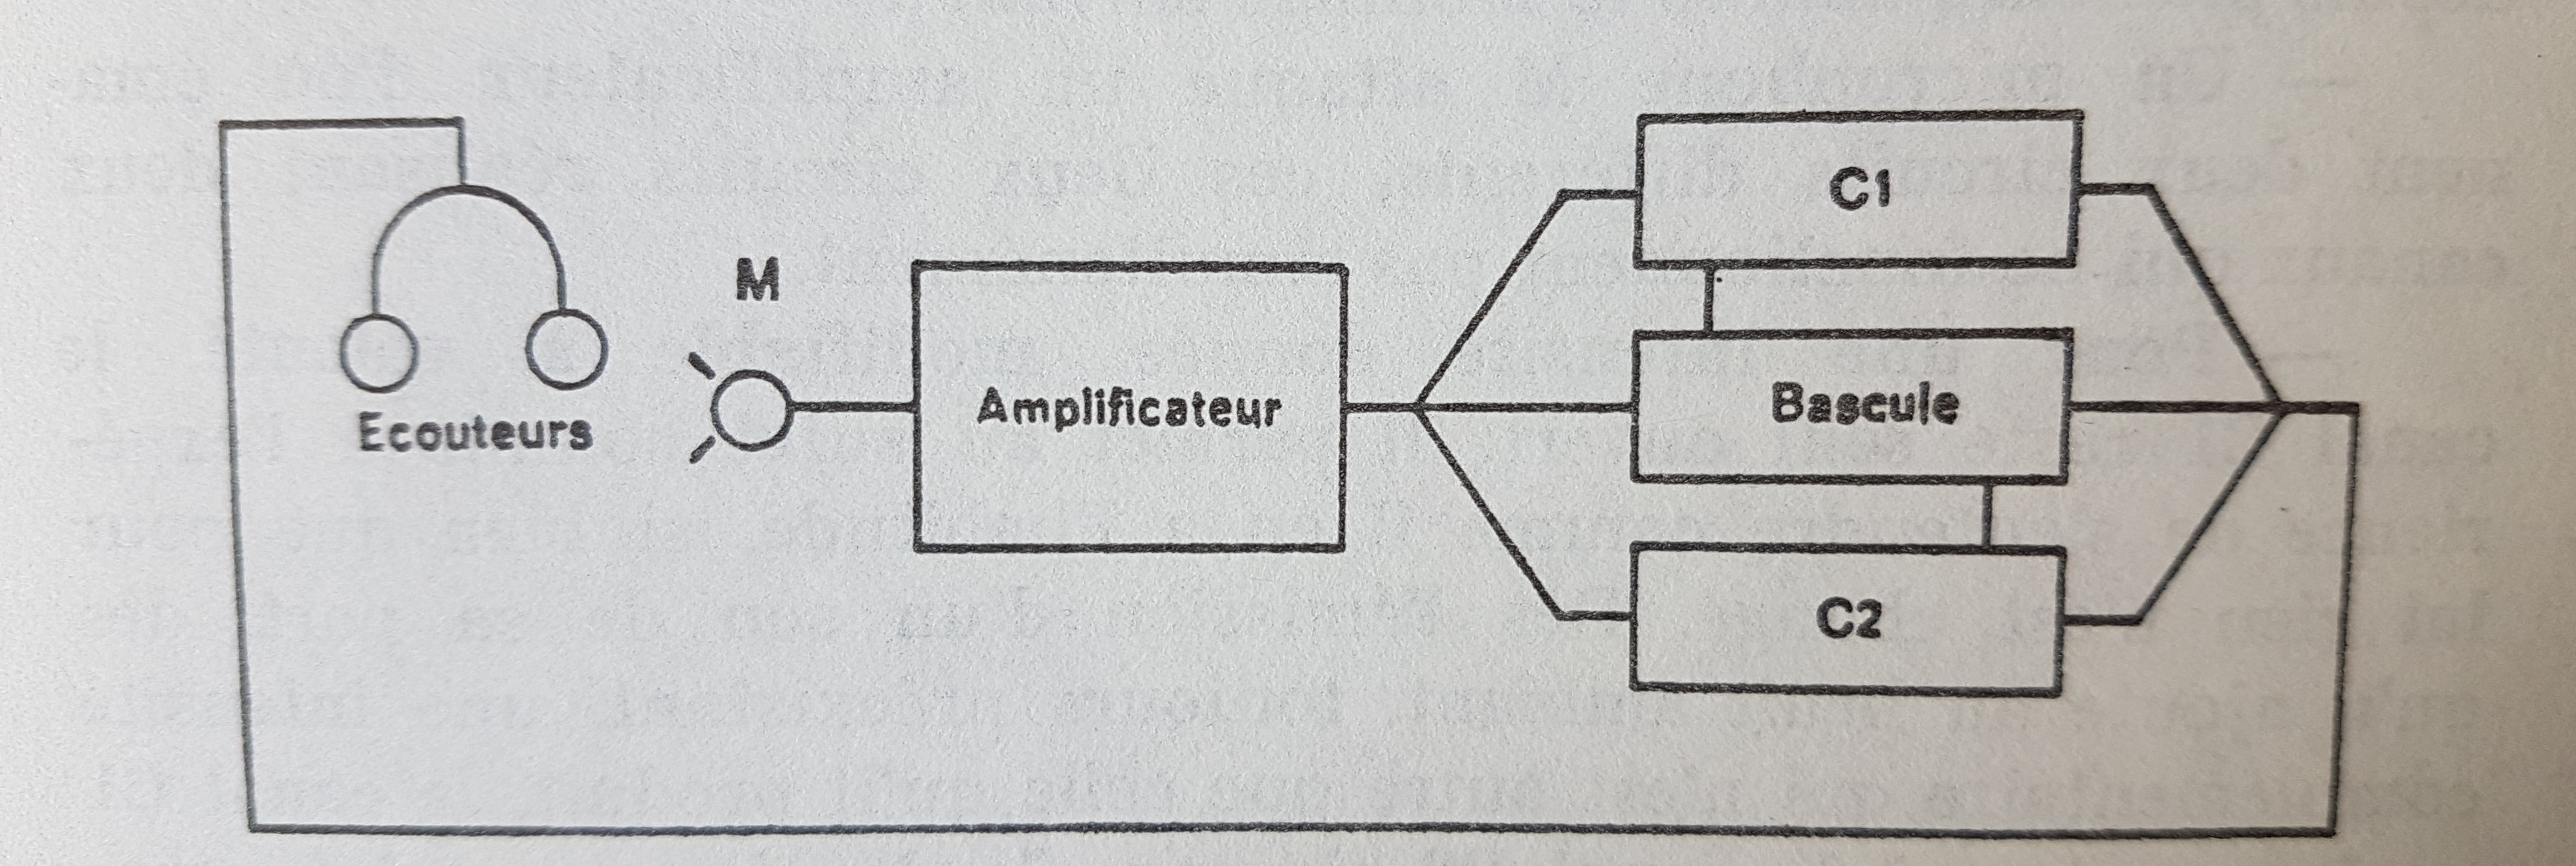
\includegraphics[width=0.7\linewidth]{images/oreilleelectro.jpg}
	\caption[L'Oreille
          Electronique: schéma]{Schéma initial de l'Oreille
          Electronique,\autocite[p.~97] {tomatisoreilletvie}}
\label{oreilleelectro}
\end{figure}
En fait, ce schéma comprend le\textit{ feed-back}, un des principes
cybernétiques lié au concept de l'\textit{homéostasie} tel
mentionné dans le dictionnaire de
psychologie \autocite[298]{doronparot}.
% \footnote{Doron et Parot, rétroaction;
  %feedback positif = il faut varier, f.négatif= ne rien faire,  feed-back, Doron/ Parot, .p177 : cybernétique. Concept de l'homéostasie, Cannon}
En effet, dès les premières
séances, Tomatis constate une amélioration temporaire de la voix, se
stabilisant avec l'entraînement, et établissant ainsi le
\textbf{lien frappant} entre\textbf{ l'écoute et
  l'émission vocale} \autocite {tomatisoreilletvie}.

De même, la façon d'émettre un son, le timbre de la voix et la fluidité
verbale figurent parmi des
éléments clairement significatifs en musicothérapie.
%La façon dont vont évoluer ces paramètres observables
Un test d'écoute peut, par observation et comparaison, donner des informations sur la manière dont vont évoluer ces paramètres, au fil d'une thérapie mais aussi et surtout à son aboutissement, et c'est ce que nous allons aborder plus loin.


%Par cette brève introduction, nous pouvons ainsi mieux percevoir l'importance que Tomatis donnait à l'oreille, donc à l'écoute et à ses recherches pour accompagner le patient dans sa thérapie.
%La recherche d'harmonie, d'équilibre et de bien-être du patient sont les buts et les résultats auxquels toute thérapie tend.
%Etre à même de percevoir le sujet là où il se tient, de comprendre ses blocages ou sa problématique, n'est pas toujours tâche facile.
%Si à l'issue d'une thérapie des difficultés subsistent, une distorsion décelée grâce à un test d'écoute peut amener un élément de réponse.
%comme un repli comportemental, un refus de sons, une disto
%Le but de toutes thérapies, y compris celle de la musicothérapie est

%de faire prendre conscience de certaines problématiques afin de faire accéder le patient à un mieux-être, voire à une forme d'harmonie.

  %Parfois, nous pouvons nous heurter
 %dans le but ultime de son épanouissement, accédant ainsi à une forme d'harmonie.
%permettant au patient d'accéder
%mais aussi à la qualité vocale et instrumentale.
